\documentclass[sponsored]{acmsiggraph}

\title{Developing a Marble game \\ \large \normalfont Results of a practical
course at the Chair for Computer Graphics and Multimedia \\ (RWTH Aachen
University, Germany)}

\author{Jasper Veit Manousek\thanks{Jasper.Manousek@rwth-aachen.de} 
\and    Steffen F\"undgens\thanks{Steffen.Fuendgens@rwth-aachen.de} 
\and    Fabian Klemp\thanks{fabian.klemp1@rwth-aachen.de} 
\and    Simon Froitzheim\thanks{simon.froitzheim@rwth-aachen.de} }

\pdfauthor{Jasper Veit Manousek, Steffen F\"undgens, Fabian Klemp, Simon Froitzheim}

\keywords{game programming, pinball game}

\usepackage{tabularx}

\begin{document}

\teaser{
  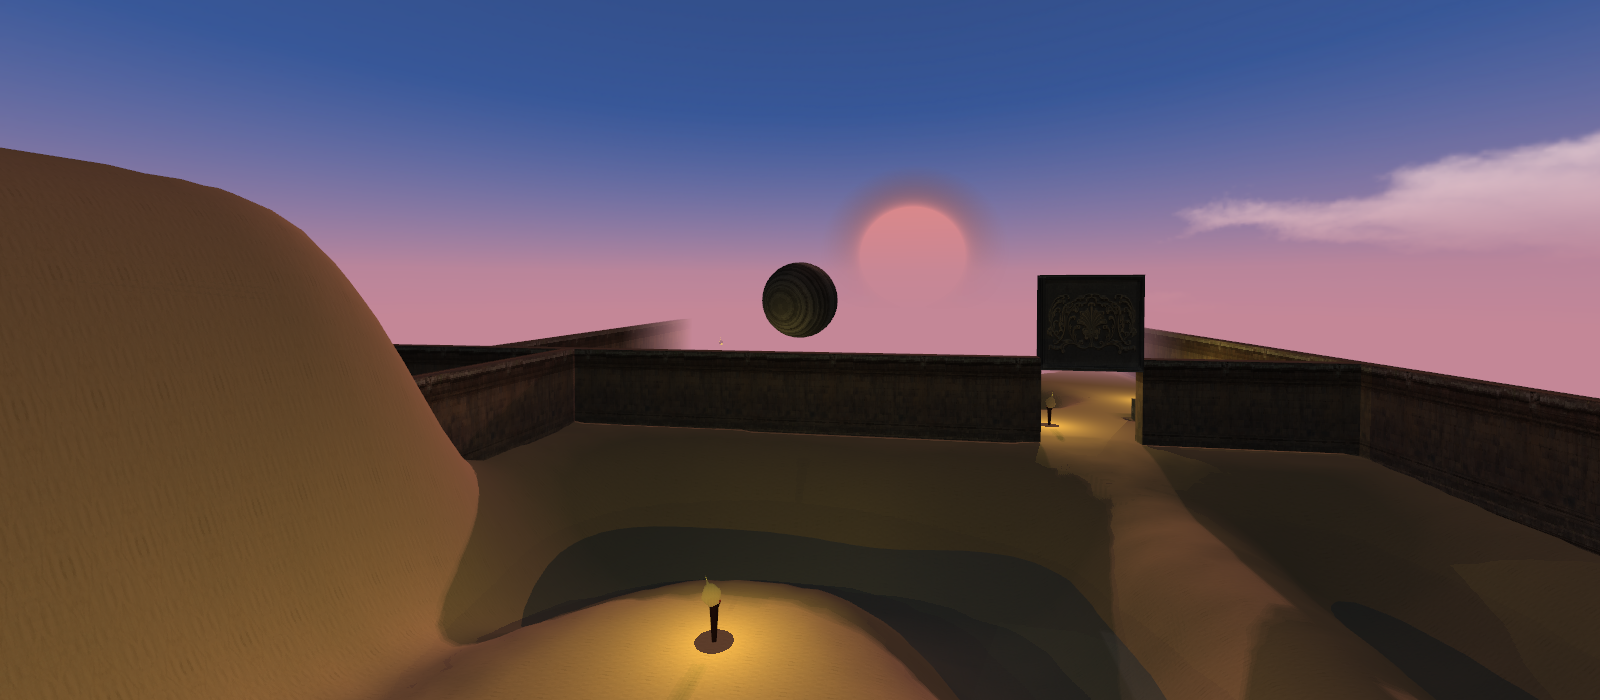
\includegraphics[width=\linewidth]{images/teasersmall.png}
  \caption{\label{fig:Teaser} Teaser}
}

\maketitle

\begin{abstract}

Marble racing games are a sub-genre of games where the player controls a marble to either run races, solve puzzles or complete some other tasks. In Saxum the player must travel through an open level completing some basic switch tasks and a simple puzzle to help the sun rise again.
 
\end{abstract}

\section{Basic Layout}

Our game is designed around the main level class. In it we load all the data from our XML files as needed. From here we also have access to the other two main classes, the physics and the graphics classes. Additionally we have the list of all our objects here.

\section{Details}

\subsection{Loading}

Our game plays mainly on a height-map. We load the height-map from a greyscale png and pass the height-data to a framebuffer, so ACGL can render it. We also pass the height-data to \textit{Bullet Physics}, to create a colision shape.

On the height-map we place objects that we load from two XML files. The compositions file defines some properties for classes of objects, like the names of the obj file and the texture file, and parameters for lighting and for the physics. It also defines compositions that are made up of multiple objects that can be scaled, rotated and translated individually. One compositions file could get used for multiple levels. The level XML file defines which compositions are placed where. This part of the file gets generated by our converter. In addition to that, the compositions can also be scaled and rotated manually here.

The converter is a separate executable that takes the path to a PNG file as input. In the PNG file compositions are placed as pixels.
We decided to let the red value of the pixel identify which kind of composition it is. The green and blue values are written by the converter and used to identify single compositions. This way manual changes in the generated level XML can be kept when the converter is run again.

\subsection{Triggers}

Because a lot of the gameplay in Saxum is focused on solving challenges and activating events, we decided to integrate the scripting language Lua to make our triggers customizable. In the level XML we can add triggers to objects. We define a region in global space and when the object enters or leaves the region a Lua script is called. The script can then activate different events like opening a door or letting the sun rise at the end of the level.

\subsection{Graphics}

For the visual aspects we started with basic rendering of OBJ files. Every object has a position and a rotation.
The loading of the OBJ files and the textures was already implemented in ACGL.
Next we implemented Phong shading for point lights and directional lights.
This gave us a basic lighting model, based on the normals of the triangle meshes.

We then moved on to shadow mapping for shadows.
We started with shadow mapping for our only directional light(the sun), because it was the easiest to implement.
To further refine our shadows we implemented Cascaded Shadow Mapping, which utilizes several shadow maps with different
resolutions(the closer to the camera, the higher the resolution).

Later we expanded on this by implementing shadow mapping for point lights using cube map textures. It took quite some time to implement them correctly due to
discrepancies of how OpenGL defined the up vector and how we thought it should be.

We implemented a basic day/night cycle using one sky texture for the day and one for the night which get blended together depending of the height
of the sun.

The sky textures were mapped on a skydome and the sun was procedually painted on top. This allowed the sun to easily be moved during runtime.

To hide the popping of object and the terrain into the view frustum we implemented a basic fog.
We later changed the color of the for depeding of the sun height to get a more realistic sun rise.

The last feature we implemented was a basic flame rendering. 
To do that we used a geometry shader to generate a basic flame shape during runtime.
The circular flame shape is generated using a cosine and a exponential function.

To get a simple illusion of heat we blurred the flames:
We do this in several render passes:
At first we render the flames with color.
After that we increase the size of the flames a little bit and render the flames without color while also writing to the stencil buffer.
We then blur the parts selected by the stencil shader.

\subsection{Physics}

The physics is based on Bullet Physics, with a simple callback function used to relay the data to the graphics pipeline. We decided to use  a btvhTerrainShape for the terrain. This is much more effective than using a triangle mesh. Additionally we have spheres, boxes, and a few other basic primitives. Finally we implemented btvhTriangleMesh shapes and concave triangle meshes, which are more strenuous for the system, but allow for moveable triangle meshes.

Unfortunately Bullet Physics proved unable to handle many forms of constraints that we required. For this we created two instances of spring constraints. The first is a spring constraint which creates a force attempting to keep two rigid bodies a set distance apart. The second was a derivation of the first, generating a force in an attempt to confine the rigid body to a certain position. This constraint is what we used to create switches that could be embedded within the terrain by filtering out the collision between the two bodies.
We also used a similar constraint to create a physics based camera. The camera attempts to follow the player at an angle specified by the player. Finally we used the constraints to get the player to float in the air. To do this a constraint is added via the LUA script, allowing the player get an improved view of the sunrise.

Additionally the respawn animation was created using the physics engine. It lets the ball continue to rotate, while changing certain properties of it, especially how it will move and that it will ignore the collision with all other objects. After it sinks a certain distance it will reappear in a similar fashion before its normal physic state is restored.

The physics came with many challenges, partially stemming from our integration into a new field, but also partially due to the nature of Bullet Physics itself. If bullet does not recieve enough updates the simulation becomes jagged and unrealistic. To solve this it is suggested to recall the world multiple times per frame to allow a more accurate simulation. Unfortunately, especially with the introduction of the physics based camera, problems arose. To solve this we not only recalled the complete update method within the physics, but also recall the complete update method in the level to stabilize the experience.

\subsection{Content Creation}

\section{Conclusion}

Our group had no prior experience with such large projects. Though our lack of previous experience hampered our progress, we have managed to amass a great deal of experience in game design, project management and teamwork, as well as knowledge in the underlying framework of games.

Our game is an interesting twist on an old concept, and our play tests have shown that we manage to achieve a notable awe factor for those who complete it.

Through the experience we have gained we are confident that all our future projects, especially those in the discipline of game programming will benefit greatly.



%\begin{figure}[t]
%    \centering
%    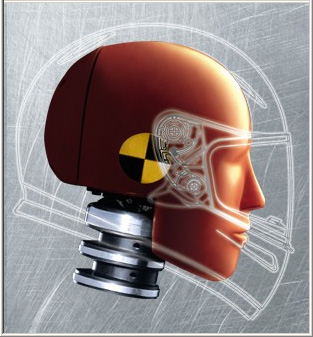
\includegraphics[width=0.3\linewidth]{images/Dummy}
%    \caption{\label{fig:OneImage} Use one image.}
%\end{figure}
%
%\begin{figure}[t]
%    \centering
%    \parbox{0.3\linewidth}{\centering 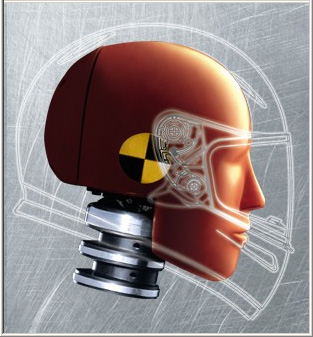
\includegraphics[width=\linewidth]{images/Dummy} \\ (a)}
%    \parbox{0.3\linewidth}{\centering 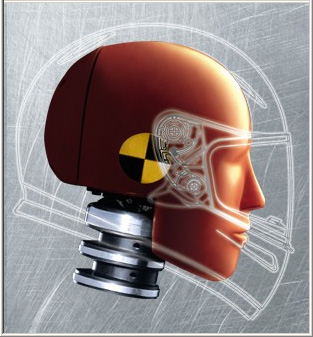
\includegraphics[width=\linewidth]{images/Dummy} \\ (b)}
%    \parbox{0.3\linewidth}{\centering 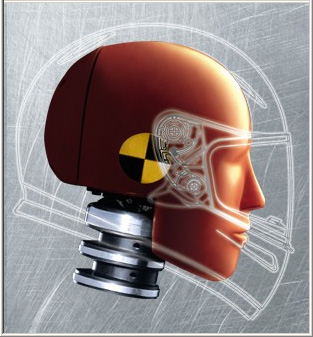
\includegraphics[width=\linewidth]{images/Dummy} \\ (c)}
%    \caption{\label{fig:SeveralImages} 
%    Use several images.}
%\end{figure}

\bibliographystyle{acmsiggraph}
\bibliography{references}
\end{document}
